\section{Descrizione del modello}

\subsection{Overview}
\begin{frame}{Approccio ad agenti}
	\begin{itemize}
		\item \textbf{Sistema multiagente} sviluppato in python con il framework Mesa
		\begin{itemize}
			\item \textbf{Ambiente}: Supermercato
			\begin{itemize}
				\item Il supermercato è una struttra divisa in zone, composto da code e casse
				\item I clienti entrano nel supermercato per fare la spesa minimizzando il tempo impiegato
			\end{itemize}
			\item \textbf{Agenti}: Clienti e casse
		\end{itemize}
	
		\item I clienti sono agenti intelligenti (pianificano e decidono) con una componente impredicibile che fa emergere un comportamento complesso interagendo con gli altri agenti
	\end{itemize}
\end{frame}

\begin{frame}{Ambiente}
	
	\begin{figure}[H]
		\centering
		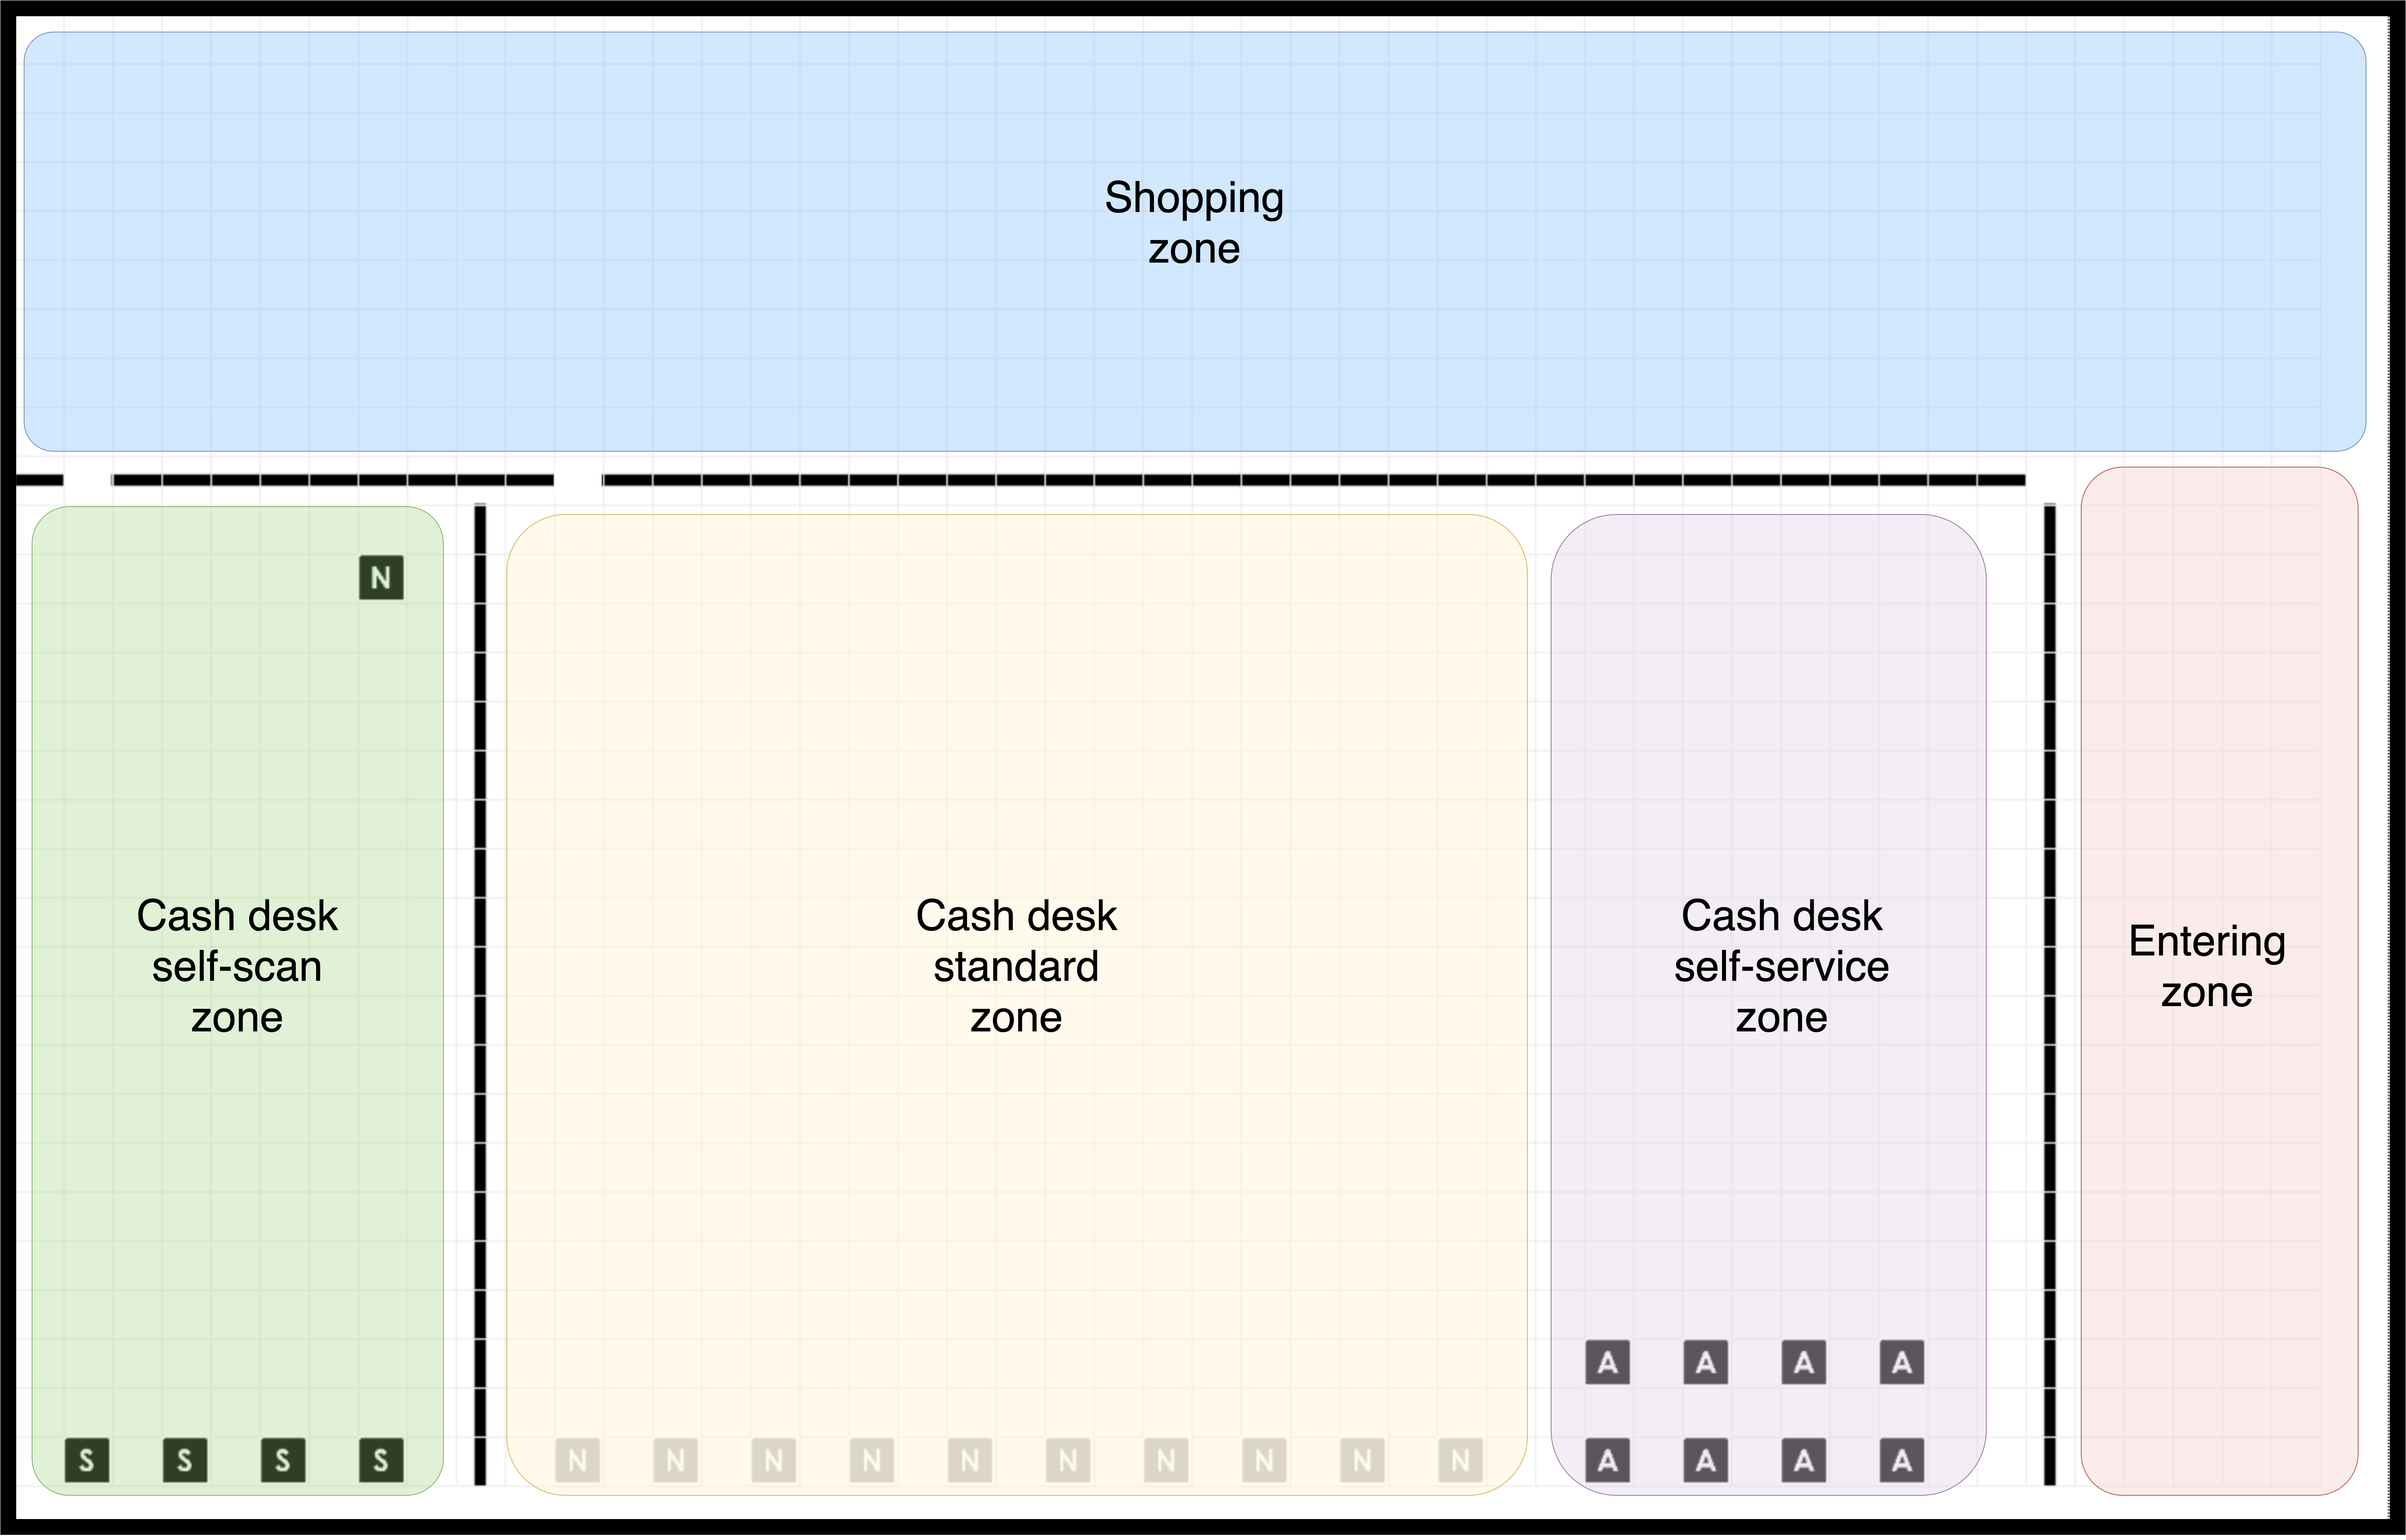
\includegraphics[width=9cm]{"../report/images/supermarket-start-zones.png"}
		\caption{Stuttura del supermercato diviso in zone.}
		\label{fig:supermarket_zones}
	\end{figure}
	
	
\end{frame}


\begin{frame}{Ambiente}
	\begin{figure}[H]
		\centering
		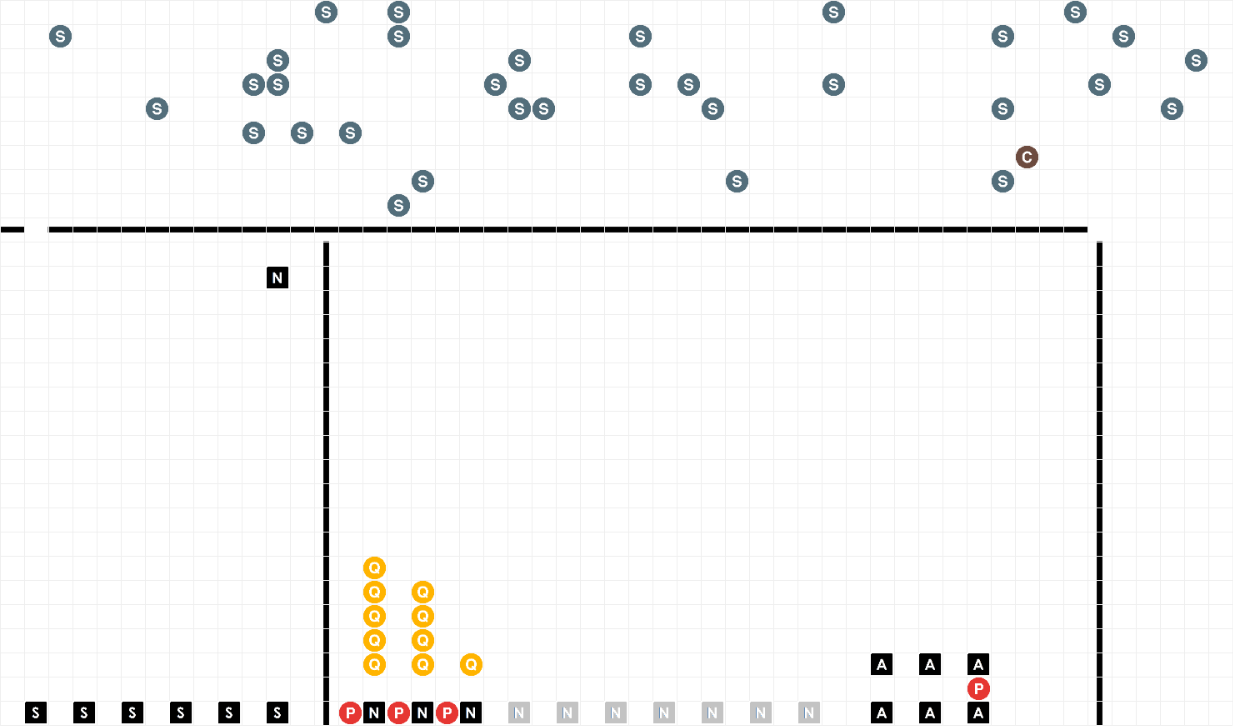
\includegraphics[width=9cm]{"../report/images/supermarket-execution.png"}
		\caption{Interzione tra agenti e abmiente.}
		\label{fig:supermarket_execution}
	\end{figure}	
\end{frame}


%----------------------------------------------------------------------------------------


\begin{frame}{Descrizione del modello}
	\centering
	Cose teoriche su ambiente, agenti, interazione
	\#TODO: Marco
\end{frame}


%----------------------------------------------------------------------------------------

\subsection{Agenti del modello}

\begin{frame}{Agente di tipo Cliente}
	\centering
	cosa fa e che tipo di agente è - workflow
	\#Todo: LLucrezia
\end{frame}


%----------------------------------------------------------------------------------------


\begin{frame}{Agente Cassa}
	\begin{itemize}
		\item I clienti, una volta conclusa la fase si di spesa, scelgono una coda in attesa di essere serviti in cassa per il pagamento.
		\item Ogni cassa ha al più una coda associata.
		\item La cassa è un'agente di tipo model based reflex, lo stato è il cliente che si sta processando in un deteminato momento.
		\item Il comportamento di una cassa è piuttosto semplice:
		\begin{enumerate}
			\item Prendi un cliente dalla coda (se disponibile)
			\item Processa il cliente
			\item Ripeti
		\end{enumerate}
		\item Le code (FIFO) ammissibili per ogni cassa sono di 2 tipi:
		\begin{enumerate}
			\item Coda dedicata: La cassa ha una coda dedicata
			\item Coda condivida: Una coda è associata a più casse, tutte le casse serviranno i clienti che si sono accodati alla coda condivisa.
		\end{enumerate}
		\item Nel modello sono state modellate 4 tipi di casse diverse.
	
	\end{itemize}
\end{frame}

\begin{frame}{Agente Cassa - Tipo 1: Standard}
	\begin{itemize}
		\item Rappresenta la classica cassa di un supermercato.
		\item Questa cassa ha una coda dedicata
		\begin{enumerate}
			\item Il cliente si accoda
			\item La cassa prende il primo cliente dalla coda
			\item Il cassiere processa gradualemnte tutti gli articoli del cliente
			\item Ripeti
		\end{enumerate}		
	\end{itemize}
\end{frame}

\begin{frame}{Agente Cassa - Tipo 2: Self service}
	
	\begin{itemize}
		\item Cassa in cui non è presente un cassiere ma è il cliente stesso a dover passare uno alla volta gli articoli acquistati.
		\item Tutte le casse self service hanno una coda condivisa
		\begin{enumerate}
			\item Il cliente si accoda alla coda condivisa
			\item La cassa prende il primo cliente dalla coda
			\item Il cliente processa ogni articolo
			\item Il cliente lascia il supermercato
		\end{enumerate}		
	\end{itemize}
\end{frame}

\begin{frame}{Agente Cassa - Tipo 3: Self scan}
	
	\begin{itemize}
		\item Il cliente scannerizza gli articoli durante la spesa mediante un dispositivo fornito dal supermercato.
		\item Avendo già scanerizzato gli articoli a priori non è necessario farlo in cassa
		\item Vengono effettuati controlli a campione per verificare il corretto comportamento dei clienti (tutti gli articoli devono essere stati effettivamente scannerizzati durante la spesa)
		\item Tutte le casse hanno una coda condivisa
		\begin{enumerate}
			\item Il cliente si accoda alla coda condivisa
			\item La cassa prende il primo cliente dalla coda
			\item Nel caso in cui il cliente è stato estratto per una rilettura della spesa si reca ad una cassa riservata, altrimenti esce dal supermercato
		\end{enumerate}		
	\end{itemize}
\end{frame}

\begin{frame}{Agente Cassa - Tipo 4: Riservata}
	
	\begin{itemize}
		\item Comportamento analogo alla cassa standard.
		\item Ha una coda dedicata.
		\item Nel caso di rilettura alla cassa "self scan", il cliente viene normalmente processato in questa nuova cassa.
		\item Nessun cliente può venire processato nella cassa riservata a meno di una rilettura.
	\end{itemize}
\end{frame}


%----------------------------------------------------------------------------------------


\begin{frame}{Considerazioni}
	\centering
	Il nostro modello è stra flessibile per le strategie e per gli stati e anche per i parametri che mo descriviamo
	\#TODO: Marco
\end{frame}


%----------------------------------------------------------------------------------------


\begin{frame}{Parametri}
	\centering
	Mega elenco puntato dei parametri (non roba matematica qui non serve)

	\#Todo: LLucrezia
\end{frame}